% ===========================================================================
\section{Results}
\label{sec:results}
% ===========================================================================

\subsection{The sector}

Pakistan's waste sector emitted \SI{37.45}{\mega\tonne} \COe{} in FY2023--24 on AR5 metrics, or
\SI{36.37}{\mega\tonne} on AR6. Domestic wastewater is \SI{65.3}{\percent} of it.

\begin{table}[htbp]
\centering
\footnotesize
\begin{tabular}{@{}llrrr@{}}
\toprule
\textbf{Category} & \textbf{Gas} & \textbf{Gg} & \textbf{Mt \COe{}} & \textbf{$\pm$\%} \\
\midrule
Open burning (4C2)        & \COtwo{} (fossil) & 1853.21 & 1.853 &  84.3 \\
                          & \CHfour{}         &   61.12 & 1.712 &  92.9 \\
                          & \NtwoO{}          &    0.99 & 0.262 & 124.2 \\
Solid-waste disposal (4A) & \CHfour{}         &  327.45 & 9.169 &  79.8 \\
Domestic wastewater (4D1) & \CHfour{}         &  781.63 & 21.886 & 73.7 \\
                          & \NtwoO{}          &    9.71 & 2.572 & 268.0 \\
\midrule
\textbf{Total}            &                   &         & \textbf{37.453} & \textbf{51.1} \\
\bottomrule
\end{tabular}
\caption{Waste-sector emissions, FY2023--24, AR5 GWP-100. Biogenic \COtwo{} from the biomass content
of burned waste, \SI{3520}{\giga\gram}, is a memo item outside the total per Vol~5 Ch~5
\S5.1. The sector band is the Approach-1 quadrature over these six components.}
\label{tab:results}
\end{table}

\begin{figure}[htbp]
\centering
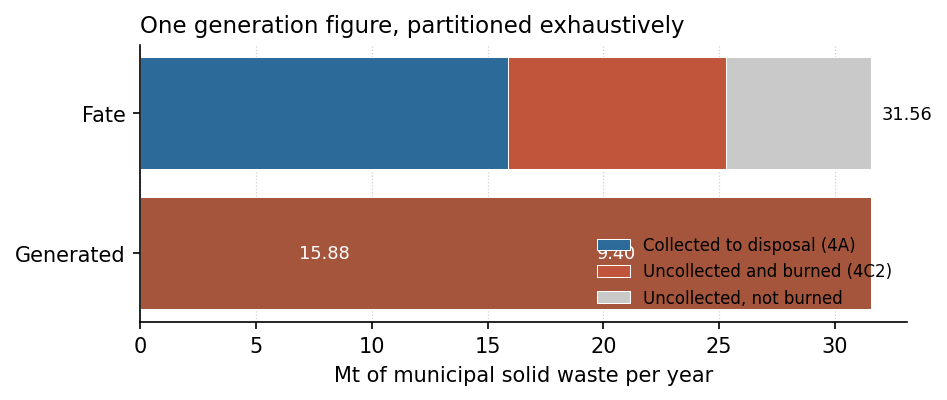
\includegraphics[width=\linewidth]{waste_partition.png}
\caption{The partition. \SI{31.56}{\mega\tonne} of municipal solid waste is generated;
\SI{15.88}{\mega\tonne} is collected and enters the decay model as 4A;
\SI{15.67}{\mega\tonne} is uncollected, of which \SI{9.40}{\mega\tonne} burns as 4C2 and the
remainder is dumped without combustion. The two lower bars sum to the upper one exactly,
which is the property the code asserts rather than checks.}
\label{fig:partition}
\end{figure}

\begin{figure}[htbp]
\centering
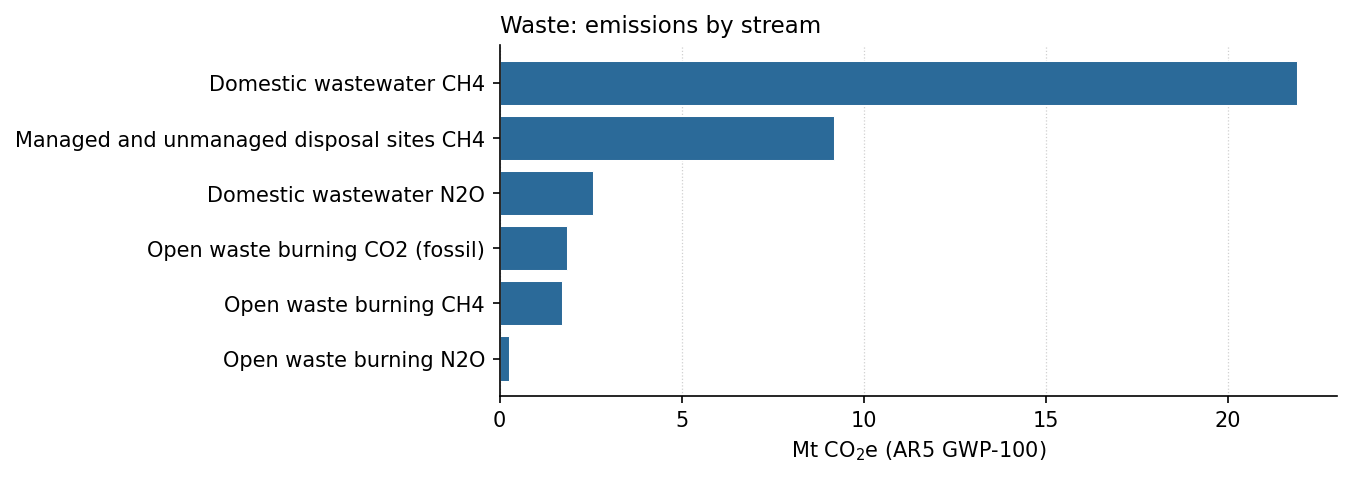
\includegraphics[width=\linewidth]{waste_streams.png}
\caption{Emissions by stream. Domestic wastewater methane alone, at
\SI{21.89}{\mega\tonne} \COe{}, is larger than the other five streams combined.}
\label{fig:streams}
\end{figure}

Methane is \SI{87}{\percent} of the sector, which is why the AR5-to-AR6 difference of
\SI{1.08}{\mega\tonne} is almost entirely a methane effect and why this sector is unusually
sensitive to the metric chosen.

\subsection{Where the uncertainty is}

The factor and activity uncertainties differ substantially by pathway. The current common ensemble reruns the native waste calculation for each realisation and preserves both the waste-fate identity and the asymmetric effluent-N$_2$O factor distribution. Its reference-year conditional interval is \SIrange{25.4}{61.5}{\mega\tonne} CO$_2$e on AR5. This is a parameter interval within the selected management interpretation and source coverage; structural cases remain separate. The standalone sector ensemble and Approach~1 screen retain their own stated settings and are not substituted for the common release interval (Supplementary Note~S1).

\subsection{Sensitivities, published rather than chosen}

\begin{table}[htbp]
\centering
\footnotesize
\begin{tabular}{@{}lrr@{}}
\toprule
\textbf{Assumption} & \textbf{Category (Mt)} & \textbf{Sector (Mt)} \\
\midrule
Sewer MCF \num{0.5} (reported)      & 24.46 & 37.45 \\
Sewer MCF \num{0.1} (river reading) & 15.39 & 28.38 \\
BOD at India's \SI{34}{} g/cap/day  & 21.17 & 34.17 \\
\midrule
Disposal with spin-up (reported)    &  9.17 & 37.45 \\
Disposal without spin-up            &  8.07 & 36.35 \\
\bottomrule
\end{tabular}
\caption{The three assumptions this sector cannot settle, each reported as an alternative
rather than absorbed into the central estimate. Nitrous oxide is invariant under both
wastewater cases because it derives from protein rather than from BOD or sewer condition, so
all rows are category totals including it---a distinction this sector's own output file
previously got wrong.}
\label{tab:sensitivity}
\end{table}

\begin{figure}[htbp]
\centering
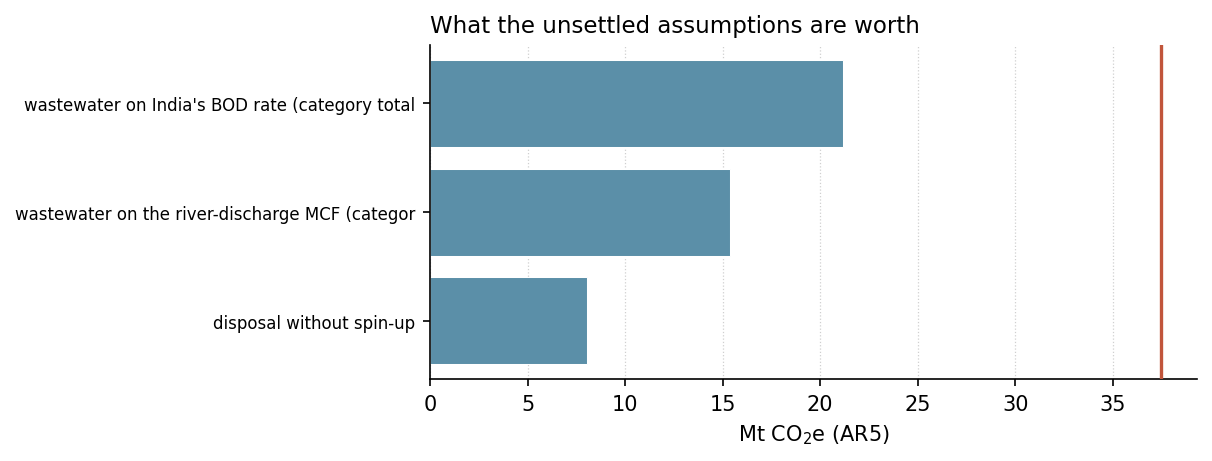
\includegraphics[width=\linewidth]{waste_sensitivity.png}
\caption{The same result as a range around the reported figure. A reader who has to
reconstruct a range from prose will not reconstruct it.}
\label{fig:sensitivity}
\end{figure}

The spin-up row answers a question most first-order-decay implementations answer implicitly:
pre-2000 deposits contribute \SI{12}{\percent} of today's landfill methane. An implementation
that starts at its activity panel is not making no assumption; it is asserting that the
country landfilled nothing before its data begin.

Named structural cases retain their own sewer and management assumptions. They are not
combined into a probability mixture. Conditional parameter intervals describe a specified
case; differences between cases remain a separate sensitivity, including the alternative
partition based on the HIES household route shares in Section~\ref{sec:validation}.

\subsection{Provincial allocation}

\begin{figure}[htbp]
\centering
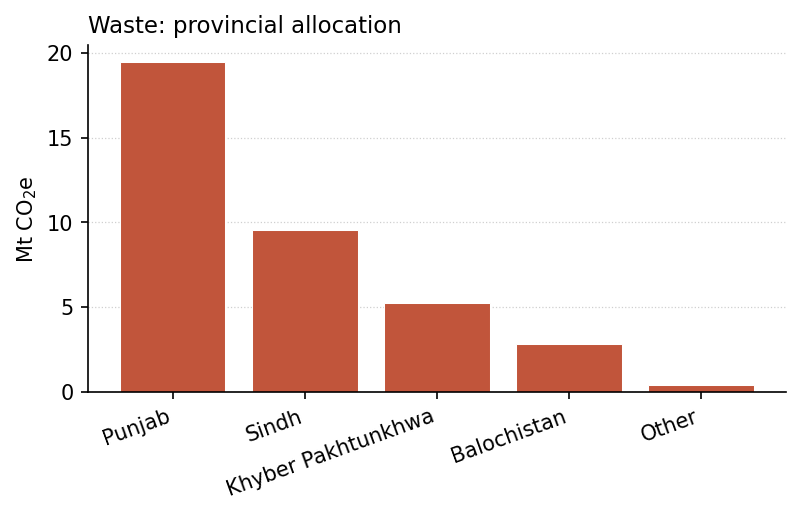
\includegraphics[width=\linewidth]{waste_provincial.png}
\caption{Punjab \SI{19.49}{\mega\tonne}, Sindh \SI{9.55}{\mega\tonne}, Khyber Pakhtunkhwa
\SI{5.21}{\mega\tonne}, Balochistan \SI{2.80}{\mega\tonne} and \SI{0.40}{\mega\tonne} in the
territories. Allocated on the same district population panel that drives generation. This is an
\emph{origin} allocation: population locates where waste and wastewater are produced, and
the split reconciles exactly against each category's national figure---but it carries the
further assumption that release is co-located with origin, which is the stronger claim.}
\label{fig:provincial}
\end{figure}

The provincial pattern follows population closely, which is expected for a sector whose
activity datum \emph{is} population, and is the reason this sector's geography is less
informative than, say, the power sector's. What the allocation locates is the \emph{origin}
of the waste and wastewater---where the generating people live---not the release: disposal
methane is emitted at landfills and dumps, wastewater methane along drains, at treatment
works and at discharge points, and burning at burn sites. What the inventory holds toward
that release geography is a prospective seed only: \num{56} OpenStreetMap
\texttt{landuse=landfill} polygons \citep{osm2026} (ODbL~1.0 derivative database,
\texttt{data/gis/landfills/}), \num{13} of them named, quality-flagged, and touched by no
estimated stream---far too sparse for an SWDS allocation, and registered so the release
can cite what it holds rather than claiming it holds nothing. The three
objects are published SEPARATELY, as the review asked: origin
(\texttt{waste\_district\_2024.csv}), fate (the ledger), and release---the polygons
republished as candidates
(\texttt{outputs/waste\_release\_candidates\_2024.csv}) with an assignment product
(\texttt{outputs/waste\_\allowbreak release\_\allowbreak assignment\_\allowbreak 2024.csv})
whose defining column is EXPLICIT UNASSIGNED MASS: a district's disposal emissions
are assigned only to its own mapped candidates (equal split, capacity unknown and
declared), nothing crosses a district boundary, and \SI{75}{\percent} of the
disposal category stays unassigned across \num{113} districts---the honest measure
of how far a release map is from existing. At provincial resolution
the origin/release distinction is modest, because waste
rarely crosses a provincial boundary between generation and fate; at any finer resolution
the population surface would place landfill methane in residential neighbourhoods, which
is why the sector's ALLOCATION remains origin-based and the limitations
section carries the gap.

\subsection{Contribution to the national inventory}

The category composition separates wastewater methane and N$_2$O, disposal-history methane and burning releases. Their uncertainty and user relevance depend on the species: a small contribution to the GHG aggregate does not imply a small primary PM or other pollutant release. The current native ensemble and pollutant-specific driver diagnostics are used to identify parameter sensitivity, without treating the old Approach~1 category screen as an additive variance decomposition of the nonlinear national ensemble.
